\documentclass[11pt]{beamer}
\usetheme{Berlin}
\usecolortheme{orchid}
\usepackage[utf8]{inputenc}
\usepackage[english]{babel}
\usepackage{amsmath}
\usepackage{amsfonts}
\usepackage{amssymb}
\usepackage{graphicx}
\usepackage{cite}
\usepackage{url}
\usepackage{hyperref}
\author{Michael Bonilla}
\title{CS 595 Project Proposal: \\ Quasi-Monte Carlo Integration using
Lattice Cubature on GPU}
%\setbeamercovered{transparent} 
%\setbeamertemplate{navigation symbols}{} 
%\logo{} 
%\institute{} 
\date{October 4, 2018} 
%\subject{} 
\begin{document}
\nocite{*}
\begin{frame}
\titlepage
\end{frame}

%\begin{frame}
%\tableofcontents
%\end{frame}

\begin{frame}<1>[label=frame1]{Introduction}
\begin{itemize}
\item Monte Carlo to used for numerical integration of high dimensional problems.
\item Traditional Monte Carlo uses pseudo random numbers (\textit{rand,randn}).
\item Branch of Monte Carlo is Quasi Monte Carlo that differs in how we chose our random inputs.
\item Guaranteed Automatic Integration Library (GAIL)
\end{itemize}
\end{frame}

\begin{frame}
\centering
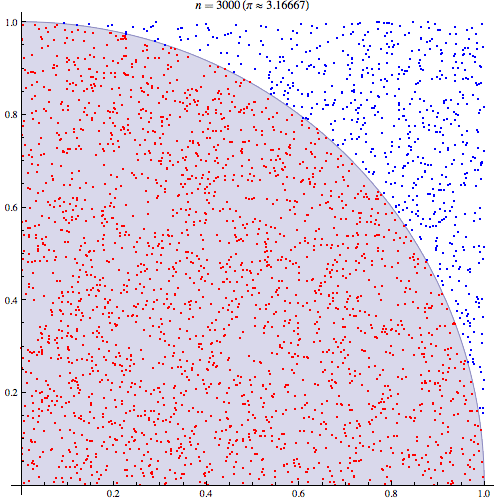
\includegraphics[width=0.7\textwidth]{mc.png} 
\end{frame}

\againframe{frame1}

\begin{frame}
\centering
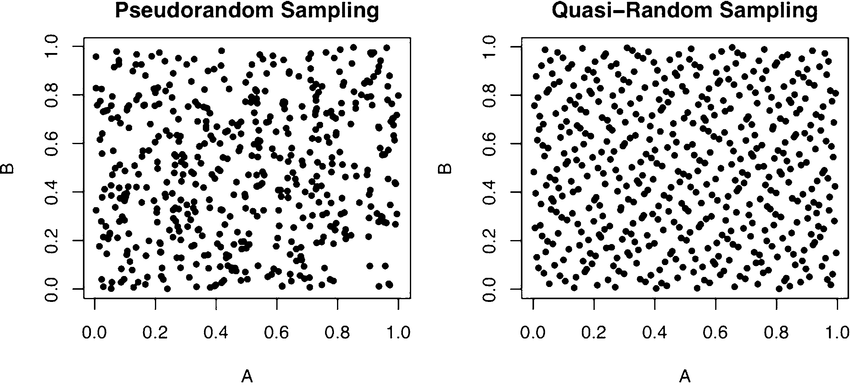
\includegraphics[width=0.7\textwidth]{pvsq.png} 
\end{frame}

\againframe{frame1}
\begin{frame}{Current Status}
\begin{itemize}
\item GAIL is written in Matlab and has no GPU capabilities.
\item Will be working on \textit{cubLattice\_g} and trying to speed it up. 
\item Currently sped up the generation of the lattices 6-8 times faster.
\end{itemize}
\end{frame}

\begin{frame}
\centering
\begin{columns}
\column{0.5\textwidth}
\centering
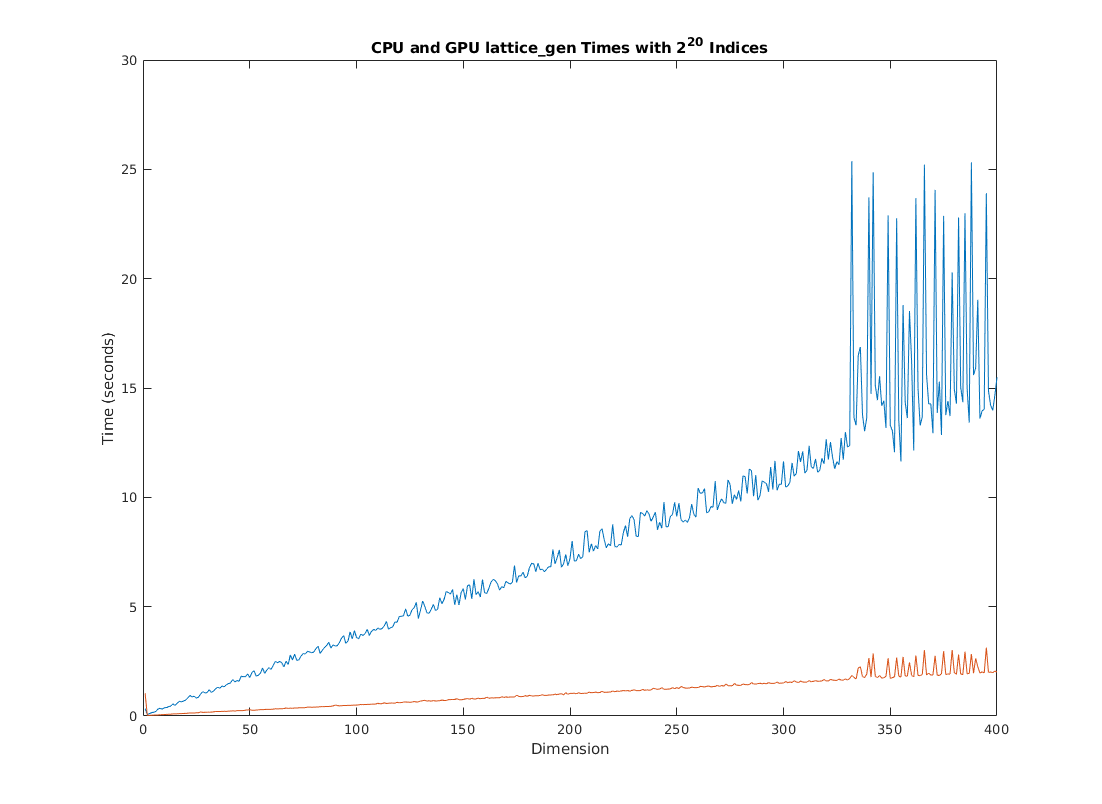
\includegraphics[width=\textwidth]{cpu_and_gpu_lattice_gen_times.png}

\column{0.5\textwidth}
\centering
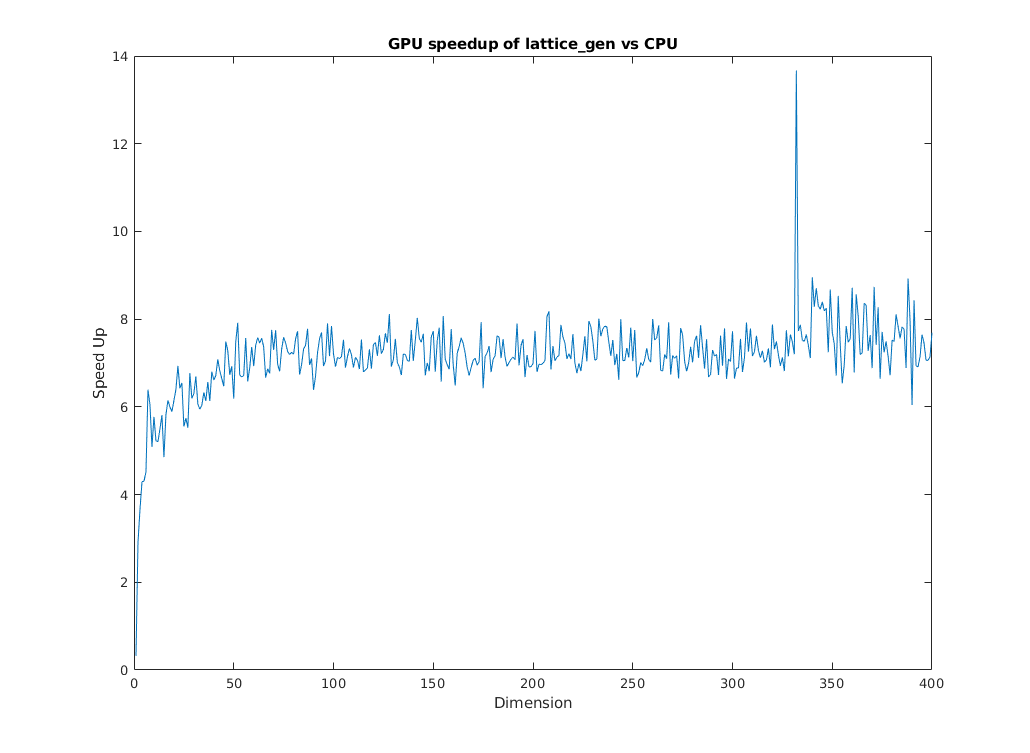
\includegraphics[width=\textwidth]{lattice_gen_speedup.png}  
\end{columns}
\end{frame}

\begin{frame}{Proposed Work}
\begin{itemize}
\item Work on \textit{cubLattice\_g} in three stages:
	\begin{enumerate}
		\item Generation of lattices in parallel.
		\item FFT of points required for algorithm.
		\item Maintain the theme of automatic integration.
	\end{enumerate}
\item Implement restrictions based on hardware.
\item testing on suitable problems of large dimension.
\end{itemize}
\end{frame}

\begin{frame}{Expectations and Further Work}
\begin{itemize}
\item Implement a GPU version of \textit{cubLattice\_g}.
\item Uphold automatic integration attributes.
\item Benchmarking of performance vs CPU
\item More robust control of GPU in Matlab
\end{itemize}
\end{frame}

\begin{frame}{References}
\bibliographystyle{abbrv}
\bibliography{cs595_references}
\end{frame}
\end{document}